\documentclass[10pt,conference]{IEEEtran}
% The preceding line is only needed to identify funding in the first footnote. If that is unneeded, please comment it out.
\usepackage{cite}
\usepackage{amsmath,amssymb,amsfonts}
\usepackage{algorithmic}
\usepackage{graphicx}
\usepackage{textcomp}
\usepackage{xcolor}
\usepackage{fancyhdr}
\usepackage{hyperref}
\usepackage[outputdir=docs]{minted}
\usepackage{amsthm}
\usepackage{ragged2e}


\hypersetup{
    colorlinks=true,
    linkcolor=blue,
    filecolor=blue,      
    urlcolor=blue,
    pdftitle={Penerapan Bilangan Acak pada Steganografi},
    pdfpagemode=FullScreen,
}

\urlstyle{same}

\def\abstractname{Abstrak}
\def\IEEEkeywordsname{Kata Kunci}
\def\refname{Daftar Pustaka}

\theoremstyle{definition}
\newtheorem{definition}{Definisi}[section]

\newtheorem{theorem}{Teorema}[section]

\def\BibTeX{{\rm B\kern-.05em{\sc i\kern-.025em b}\kern-.08em
    T\kern-.1667em\lower.7ex\hbox{E}\kern-.125emX}}

\graphicspath{{./src/img}}

%%% Footer Left
\makeatletter

\def\ps@headings{
\let\@oddhead\@empty
\let\@evenhead\@empty
\def\@oddfoot{Makalah IF2120 Matematika Diskrit – Sem. I Tahun 2021/2022\hfill}
\def\@evenfoot{Makalah IF2120 Matematika Diskrit – Sem. I Tahun 2021/2022\hfill}
}

\def\ps@IEEEtitlepagestyle{% default title page headers, no footers
\let\@oddhead\@empty
\let\@evenhead\@empty
\def\@oddfoot{Makalah IF2120 Matematika Diskrit – Sem. I Tahun 2021/2022\hfill}%
\let\@evenfoot\@empty
}
\makeatother

\pagestyle{headings}

% Document

\begin{document}

\title{Penerapan Pembangkit Bilangan Acak dalam Steganografi}

\author{\IEEEauthorblockN{Bayu Samudra - 13520128\textsuperscript{1}}
\IEEEauthorblockA{\textit{Program Studi Teknik Informatika} \\
\textit{Sekolah Teknik Elektro dan Informatika}\\
Institut Teknologi Bandung, Jl. Ganesha 10 Bandung 40132, Indonesia \\
\textsuperscript{1}13520128@std.stei.itb.ac.id}
}

\maketitle

\begin{abstract}
Steganografi adalah ilmu yang mempelajari cara untuk menyembunyikan data. Steganografi memiliki banyak cara, salah satunya adalah menggunakan
metode LSB dengan penempatan acak. Penempatan dilakukan berdasarkan hasil yang dikeluarkan oleh pembangkit bilangan acak LCG. Kelebihan dari
penggunaan ini adalah mudahnya dalam implementasi, data yang disimpan lebih tersamarkan  saat pengujian menggunakan steganalisis visual,
dan adanya sebuah kunci pengaman data yang disimpan melalui umpan dari pembangkit bilangan acak. Kelamahan dari metode ini adalah data yang disimpan
sangat mudah rusak, mudah terdeteksi dengan melakukan steganalisis statistik, mudahnya kunci ditemukan dengan menggunakan \emph{brute-force}.
\end{abstract}

\begin{IEEEkeywords}
Keamanan, Steganografi, \emph{Linear Congruetial Generator} (LCG)
\end{IEEEkeywords}

\section{Pendahuluan}
Dunia saat ini telah memasuki era yang penuh dengan data. Data setiap waktunya bertumbuh secara ekponensial. 
Data merupakan hal yang sangat penting bagi setiap orang. Data yang tersebar pada internet banyak jenisnya. 
Ada data yang merupakan data yang memang dibagikan untuk publik bahkan ada juga sata rahasia yang bersifat privat. 
Data yang bersifat privat ini haruslah dijaga kerahasiaannya. Sealh satu cara untuk menjaganya adalah dengan menggunakan kriptografi.

Kriptografi adalah ilmu yang mempelajari mengenai cara-cara untuk menjaga integritas dan keamanan dari suatu data.\cite{b1}
Dalam menjaga data, kriptografi menggunakan cabang-cabang ilmu matematika terutama dalam teori bilangan. 
Kriptografi juga merupakan sebuah seni. Hal ini dikarenakan pada awal kemunculannya, setiap orang memiliki 
caranya tersendiri untuk mengamankan pesannya. Terdapat banyak kriptografi klasik seperti Caesar Cipher, 
Vigenere Cipher, Affine Cipher, dan lainnya.

Selain menggunakan kriptografi, terdapat sebuah teknik lain untuk mengamankan sebuah data. Teknik ini dikenal steganografi. 
Steganografi adalah sebuah ilmu yang mempelajari teknik-teknik bagaimana menyembunyikan sebuah data dalam sebuah media sehingga 
sulit untuk dikenali. Steganografi ini sudah dikenal cukup lama sejak sejak bangsa Yunani. Steganografi yang pernah 
tercatat pada zaman itu adalah saat penguasa bernama Histaiaeus, seorang penguasa Yunani, mengirimkan pesan tersembunyi kepada 
Aristagoras untuk melawan Persia. Sang penguasa mengirimkan pesan tersebut dengan membotaki para budah dan rambutnya dibiarkan tumbuh, 
lalu dikirimkanlah kepada Aristagoras. Hal ini dapat dilihat pada buku yang telah ditulis oleh Herodatus, \emph{Histories of Herodatus}. \cite{b1}

Steganografi ini berbeda dengan Kriptografi. Pada kriptografi, data diubah menjadi sesuatu yang sulit dipahami makna pesan yang ada didalamnya. 
Akan tetapi, data tersebut masih ada keberadaanya. Dalam Steganografi, data disembunyikan dalam sebuah medium sehingga tidak terlihat 
keberadaannya. Medium ini bisa apapun, baik itu gambar, video, file, atau bahkan teks. Data pada medium ini pada akhirnya harus bisa 
diekstraksi untuk diambil pesannya.

Steganografi ini memiliki kelebihan, yaitu data yang dikirimkan tidak menarik perhatian orang lain. Steganografi ini pun dapat 
diintegrasikan dengan Kriptografi untuk meningkatkan keamanan data yang disimpan.

\section{Teori Dasar}

\subsection{Terminologi Dasar Steganografi}

Dalam Steganografi, dikenal beberapa terminologi dasar. Berikut ini adalah beberapa terminologi dasar yang perlu diketahui: \cite{b1}

\begin{itemize}
    \item Pesan tersembunyi adalah pesan yang disisipkan pada sebuah medium baik itu berupa video, image, audio, ataupun teks. 
    \item Cover adalah media yang digunakan untuk menyisipkan pesan.
    \item \emph{Stegeo-object} adalah media yang telah tersisipkan pesan tersembunyi di dalamnya.
    \item Steganalisis adalah cabang ilmu yang membahas mengenai pendeteksian pesan tersembunyi yang ada pada sebuah media. Terdapat 
    beberapa jenis metode dalam steganalisis ini yang akan dijelaskan pada bagian selanjutnya.  
\end{itemize}

\subsection{Kriteria Kualitas Steganografi}
Sebuah steganografi dikatakan memiliki kualitas yang baik apabila mengikuti beberapa kriteria berikut: \cite{b1}

\begin{itemize}
    \item \emph{Impercepibility} yaitu perubahan oleh steganografi tidak boleh dapat dirasakan oleh inderawi. Hal ini ditujukan agar
    tidak menimbulkan kecurigaan orang lain.
    \item \emph{Fidelity} yaitu perubahan oleh steganografi tidak jauh mengurangi kualitas dari suatu cover. Misalkan pada cover gambar,
    steganografi tidak boleh membuat gambar tersebut menjadi pecah.
    \item \emph{Recovery} yaitu pesan yang disisipkan oleh proses steganografi haruslah bisa diekstraksi kembali.
    \item \emph{Payload} yaitu pesan yang disisipkan dapat dimuat sebanyak mungkin.
    \item \emph{Robustness} yaitu \emph{stegeo-object} harus tahan terhasap serangan padanya. Akan tetapi, aspek in
    tidak terlalu dipentingkan karena steeganografi menyembunyikan pesan sehingga tidak menimbulkan kecurigaan.
\end{itemize}

\subsection{Jenis Steganalisis}
Steganalisis terbagi menjadi beberapa jenis. Berdasarkan kespesifikannya, steganalisis dibagi menjadi dua jenis, yaitu sebagai berikut \cite{b1}
\begin{itemize}
    \item \emph{Targeted Steganalysis} yaitu steganalisis yang membatasi analisis pada media atau algoritma steganografi tertentu. 
    \item \emph{Blind Steganalysis} yaitu steganalisis yang menganalisis dari berbagai algoritma dan format media. Hasil statistik dar
    setiap data akan dibandingkan dan diambil kesimpulan.
\end{itemize}

Selain berdasarkan kespesifikannya, steganografi juga dibagi menjadi menjadi dua berdasarkan metode yang digunakan.
\begin{itemize}
    \item \emph{Visual Steganalysis} yaitu steganalisis yang dilakukan dengan indera visual. Steganalisis jenis ini bersifat sujektif.
    \item \emph{Statistical Steganalysis} yaitu steganalisis yang menganalisis menggunakan analisis matematika terutama menggunakan statistika.
\end{itemize}

\subsection{Representasi Bilangan Bulat}
Pada dasarnya, komputer menyimpan dan memproses informasi dalam bentuk sinyal duanilai. Setiap sinyal tersebut merepresentasikan angka 
dalam bentuk bit. Kumpulan dari berbagai bit dapat memberikan makna dari suatu data  yang sedang diproses. Kumpulan dari berbagai bit ini 
dapat membantuk sebuah bilangan yang disebut dengan bilangan biner.

Dalam dunia keinformatikaan, terdapat dua jenis representasi bilangan bulat yang sering digunakan yaitu sebagai berikut:
\begin{itemize}
    \item \textbf{Bilangan Biner} \\
    Bilangan biner yaitu bilangan dengan basis dua. Bilangan biner hanya terdapat dua simbol yang tersedia, yaitu 0 dan 1. Konversi bilangan 
    biner ke bilangan desimal didefinisikan pada persamaan 1.
    
    \begin{equation}
         d = \sum_{i=0}^{n} b_i \cdot 2^{i}
    \end{equation}

    Nilai $ b_i $ melambangkan digit biner ke-i dan $ d $ adalah bilangan desimal hasil konversi. \\


    \item \textbf{Bilangan Hexadesimal} \\
    Bilangan Hexadesimal adalah bilangan dengan basis 16. Dua digit dari bilangan ini merepresentasikan satu byte (8-bit). Bilangan Hexadesimal 
    ini dapat meringkas penulisan biner dan juga memudahkan alam penganalisisan bilangan biner. Bilangan hexadesimal ini pada dasarnya terdiri 
    dari simbol 0 sampai dengan 9 dilanjutkan dengan simbol A,B,C,D,E, dan F. Berikut ini adalah rumus konversi bilangan heksadesimal ke bilangan desimal.

    \begin{equation}
        d = \sum_{i=0}^n h_i \cdot 16^{i}
    \end{equation}

    Nilai $ h_i $ menyatakan digit hexadesimal ke-i. Bila digit Hexadesimal bernilai $ \text{A} $ maka digantikan dengan nilai $ 10 $. Begitu 
    pula dengan nilai $ \text{B} $ yang digantikan dengan nilai 11. Hal ini berlaku seterusnya hingga $ \text{F} $.
\end{itemize}

\subsection{Signifikansi Bit}
Terdapat dua buah definisi yang perlu diperhatikan mengenai signifikansi bit.Misalkan terdapat sebuah bilangan bulat dengan $ w $-digit dan urutan 
digitnya adalah $ [b_{w-1}, b_{w-2}, \cdots, b_{2}, b_{1}, b_{0}] $. Digit $ b_{w-1} $ disebut sebagai \emph{most significant bit} atau biasa disingkat 
sebagai MSB. Bit $ b_{0} $ disebut sebagai \emph{least significant bit} atau biasa disingkat sebagai LSB.

\begin{figure}[htbp]
    \centerline{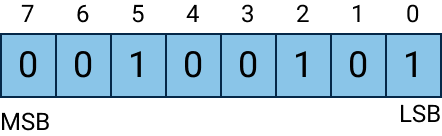
\includegraphics[width=0.9\columnwidth]{MSB-LSB.png}}
    \caption{Ilustrasi MSB dan LSB}
\end{figure}

\subsection{Citra Digital}
Pada komputer sebuah citra digital disimpan dalam kumpulan byte data. Bagian terkecil dari sebuah citra digital disebut dengan pixel. Citra digital
merupakan matriks dari pixel tersebut. Setiap pixel direpresentasikan dengan bilangan $n$-bit. Berdasarkan jumlah bit pada pixel, citra digital dapat 
diklasifikasikan menjadi beberapa jenis yaitu sebagai berikut: \cite{b1}\cite{b3}

\begin{itemize}
    \item \textbf{Citra 24-bit}\\
    Pada citra 24-bit, setiap pixel terdiri atas 3 buah kanal. Kanal pada citra ini adalah yaitu R (\emph{Red}), G (\emph{Green}), dan B (\emph{Blue}).
    Setiap kanal memiliki besar 8-bit yang merepresentasikan bilangan 0 sampai 255.

\begin{figure}[htbp]
    \centerline{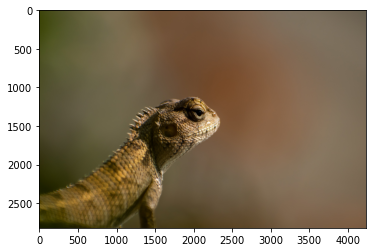
\includegraphics[width=0.9\columnwidth]{citra-original.png}}
    \caption{Citra berwarna 24-bit (Sumber: Unsplash)}
    \label{fig:24original}
\end{figure}

    \item \textbf{Citra 8-bit} \\
    Citra ini biasa disebut sebagai citra grayscale. Citra ini hanya memiliki 1 buah kanal yang menyatakan nilai keabuan. Konversi dari citra berwarna
    menjadi citra grayscale ini dapat dilakukan dengan rumus pada persamaan \ref{eq:gscvt}.

    \begin{equation} \label{eq:gscvt}
        y = 0.299 \cdot R + 0.587 \cdot G + 0.144 \cdot B
    \end{equation}

    Citra pada figur \ref{fig:8grayscale} adalah hasil konversi citra pada figur \ref{fig:24original} menjadi grayscale.

    \begin{figure}[htbp]
        \centerline{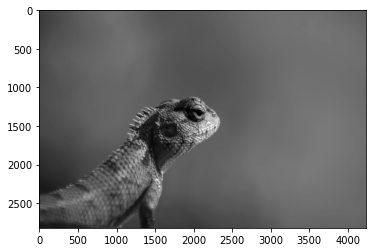
\includegraphics[width=0.9\columnwidth]{citra-gs.png}}
        \caption{Citra berwarna 8-bit)}
        \label{fig:8grayscale}
    \end{figure}

    \item \textbf{Citra 1-bit} \\
    Citra 1-bit ini biasa dikenal dengan citra biner. Citra ini hanya memiliki dua kemungkinan nilai pixel, yaitu 0 atau 1. Jenis citra ini biasa digunakan
    sebagai \emph{masking} dalam pengolahan citra. Citra pada figur \ref{fig:1binary} adalah hasil konversi pada citra figur \ref{fig:24original} menjadi citra biner.

    \begin{figure}[htbp]
        \centerline{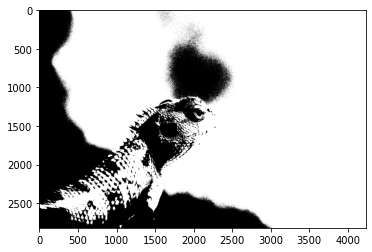
\includegraphics[width=0.9\columnwidth]{citra-bin.png}}
        \caption{Citra berwarna 1-bit}
        \label{fig:1binary}
    \end{figure}

\end{itemize}

\subsection{Luminans Relatif}
Tingkat Luminans Relatif sebuah warna ini dapat dihitung menggunakan persamaan \ref{eq:lum}.\cite{w1}

\begin{equation} \label{eq:lum}
    L = 0.2126 R_p + 0.7152 G_p + 0.0722 B_p
\end{equation}

yang dalam hal ini

$$ 
X_p = \begin{cases}
    \frac{X_r}{12.92}, &\text{jika } X_r \le 0.03928 \\
    (\frac{X_r+0.055}{1.055}) ^ {2.4},  &\text{jika } X_r > 0.03928 
\end{cases} 
$$

dengan $X$ adalah salah satu dari $R$, $G$, ataupun $B$.

Nilai dari $X_r$ merupakan rasio suatu kanal warna terhadap nilai maksimumnya.

\subsection{Rasio Kontras}
Rasio kontras antara dua buah warna menyatakan seberapa kontras kedua warna tersebut. Menurut W3C, tingkat
rasio kontras didefinisikan pada persamaan \ref{eq:cr}.\cite{w1}

\begin{equation} \label{eq:cr}
    R = \frac{L_1 + 0.05}{L_2 + 0.05}
\end{equation}

yang dalam hal ini $L_n$ adalah luminans relatif dari satu warna dengan $ L_1 > L_2 $.


\subsection{Keterbagian Bilangan Bulat}
Pembagian merupakan konsep penting yang menjadi dasar dari teori bilangan. Sebuah bilangan dapat membagi habis bilangan lain. Definisi dari habis dibagi dapat dilihat pada
definisi \ref{def:divided}.

\begin{definition} \label{def:divided}
    Misalkan $x$ dan $y$ adalah sebuah bilangan bulat. Dapat dikatakan $x$ habis membagi $y$ atau dinotasikan dengan
    $$ a | b $$
    jika dan hanya jika terdapat sebuah bilangan bulat $a$ yang memenuhi persamaan $ y = ax $
\end{definition}

Dalam berbagai bilangan bulat, terdapat satu kelompok bilangan bulat  yang sangat penting yaitu bilangan prima.
\begin{definition} \label{def:prime}
    Sebuah bilangan bulat $x$ dengan $x > 0$ dikatakan bilangan prima jika dan hanya jika bilangan tersebut hanyalah habis dibagi oleh $x$ dan 1.
\end{definition}

Terdapat teorema penting mengenai bilangan prima yang disebut dengan teorema fundramental aritmatik. \cite{b2}

\begin{theorem}[Teorema Fundramental Aritmatik]
    Setiap bilangan bulat positif yang lebih dari sama dengan 2 dapat dinyatakan sebagai perkalian yang setidaknya terdapat sebuah bilangan prima. 
\end{theorem}

Setiap bilangan prima yang dapat membagi sebuah bilangan bulat disebut dengan faktor prima.

\subsection{Aritmatika Modulo}
Dalam teori bilangan dikenal sebuah operasi yang disebut dengan operasi aritmatika modulo. Aritmatika modulo ini memainkan peran penting dalam Kriptografi untuk membantu
mengamankan data. Operator yang digunakan pada operasi modulo adalah $ \text{mod} $. Operasi ini didefinisikan pada definisi \ref{def:modulo}.

\begin{definition} \label{def:modulo}
    Misalkan $x$ dan $m$ adalah sebuah bilangan bulat dengan $ m > 0 $. Kesamaan $ x \mod{m} = r $ merupakan kesamaan semedikian sehingga $ x = ma + r $ dengan nilai $0 \le r < m$.
    Dengan kata lain, $r$ adalah sisa bagi dari pembagian $x$ dan $m$.
\end{definition}

Dalam aritmatika modulo, terkadang dua buah bilangan bisa saja memiliki hasil modulo yang sama. Kedua bilangan ini bisa disebut kongruen dalam suatu modulo. Kekongruenan ini dapat
didefinisikan sebagaimana definisi \ref{def:congruent}.

\begin{definition} \label{def:congruent}
    Misalkan terdapat tiga buah bilangan bulat $a$, $b$, dan $m$ dengan $m > 0$. Dapat dikatakan bahwa bilangan $a$ dan $b$ kongruen atau dengan notasi
    $$ a \equiv b \text{ } (\text{mod } m) $$
    jika dan hanya jika $a-b$ habis dibagi oleh $m$.
\end{definition}

\subsection{Pembagi Bersama Terbesar}
Dua buah bilangan bulat bisa saja habis dibagi dengan suatu bilangan bulat. Pembagi ini bisa saja lebih dari satu. Akan tetapi, terdapat sebuah bilangan pembagi dari kedua buah bilangan
bulat tersebut yang disebut dengan pembagi bersama terbesar (PBB) atau disebut dengan \emph{greatest common divisor} (GCD). 

\begin{definition} \label{def:gcd}
    Misalkan terdapat dua buah bilangan bulat $a$ dan $b$ dengan $a,b > 0$. Dikatakan $x$ merupakan $\gcd{(a,b)}$ jika dan hanya jika $x$ bilangan bulat terbesar yang memenuhi $x | a$ dan $x | b$.
\end{definition}

Terdapat sebuah istilah yang cukup penting, yaitu relatif prima. Dua buah bilangan bisa dikatakan relatif prima bila memenuhi definisi \ref{def:relativeprime}.

\begin{definition} \label{def:relativeprime}
    Misalkan terdapat dua buah bilangan bulat $a$ dan $b$ dengan $a,b > 0$. Dikatakan $a$ relatif prima dengan $b$ jika dan hanya jika $\gcd{(a,b)} = 1$.
\end{definition}

\subsection{Pembangkit Bilangan Acak}
Dalam dunia keinformatikaan, bilangan acak merupakan bilangan yang sangat dibutuhkan. Bilangan acak sangat diperlukan terutama dalam kriptografi. Terdapat berbagai jenis pembangkit bilangan acak,
salah satunya adalah \emph{Linear Congruential Generator} (LCG). Bilangan acak ini didefinisikan dalam relasi rekurens pada persamaan \ref{eq:lcg}.

\begin{equation} \label{eq:lcg}
    x_{i+1} = ax_{i}+b \text{ (mod }m\text{)}
\end{equation}

Untuk memulai LCG, diperlukan sebuah umpan yaitu $x_0$. Dengan umpan yang sama, dapat didapatkan sebuah nilai urutan yang sama. 
Parameter $a$, $b$ dan $m$ sangat menentukan periode dari LCG. Terdapat sebuah teorema
yang dapat membantu menentukan nilai $a$, $b$, dan $m$ agar memperoleh periode maksimum. \cite{a1}

\begin{theorem}[Teorema Hull–Dobell] \label{theo:hulldobell}
    Sebuah LCG yang didefinisikan pada definisi \ref{eq:lcg} dapat memiliki periode penuh, yaitu berperiode $m-1$ jika memenuhi syarat berikut:
    \begin{enumerate}
        \item $b$ relatif prima terhadap $m$,
        \item $a \equiv 1 \text{(mod }p\text{)}$ jika $p$ merupakan faktor prima dari $m$,
        \item $a \equiv 1 \text{(mod }4\text{)}$ jika $m$ adalah bilangan yang habis dibagi oleh 4.
    \end{enumerate}
\end{theorem}

\section{Pembahasan}
\subsection{Metode Steganografi}
Pada penelitian ini, akan digunakan metode steganografi berbasis LSB. Nilai $m$ yang digunakan adalah jumlah pixel yang terdapat pada cover. Metode penyisipan yang digunakan adalah sebgai berikut.
\begin{enumerate}
    \item Menentukan parameter $a$ dan $b$ untuk LCG.
    \item Mengubah gambar menjadi dalam bentuk matriks pixel.
    \item Mengubah matriks pixel menjadi array lanjar agar lebih mudah untuk diolah.
    \item \label{step:1} Menentukan angka acak dengan menggunakan LCG.
    \item Mengambil $n$ bit dari lsb dari data yang akan disisipkan, lalu menimpa pada array lanjar. 
    \item Kembali melakukan dimulai dari langkah \ref{step:1} hingga semua data yang akan disisipkan sudah dimasukan atau tidak tersedia ruang untuk menambahkan data baru.
    \item Menambahkan string \mintinline{python}{"\x00"} pada array lanjar dengan menggunakan angka acak selanjutnya. Langkah ini dilakukan apabila ruang untuk memasukan data ini masih tersedia.
\end{enumerate}

Langkah yang dilakukan untuk mengekstraksi data pada \emph{stegeo-object} adalah sebagai berikut:
\begin{enumerate}
    \item Menentukan parameter $a$ dan $b$ untuk LCG.
    \item Mengubah gambar menjadi dalam bentuk matriks pixel.
    \item Mengubah matriks pixel menjadi array lanjar agar lebih mudah untuk diolah.
    \item \label{step:2} Menentukan angka acak dengan menggunakan LCG.
    \item Mengambil $n$ bit dari lsb array lanjar pada indeks yang ditunjukan oleh hasil LCG. Kumpulkan hingga mendapatkan 8-bit. Pengumpulan menggunakan aturan little endian.
    \item Bila telah mencapai 8-bit, ubahlah bit yang telah dikumpulkan menjadi karakter.
    \item Lakukan kembali dimulai langkah \ref{step:2} hingga didapatkan 1 byte yang bernilai 0. Hasil itu menjadi penanda bahwa proses telah berakhir.
\end{enumerate}

Jumlah $n$ yang disarankan untuk melakukan proses ini adalah $n$ yang memenuhi $n = 2^k$ dengan $k$ adalah bilangan bulan dan $k \le 8$. Hal ini dilakukan agar mendapatkan kelipatan 8 setiap iterasi saat melakukan
ekstraksi pesan.

\subsection{Pemilihan Parameter}
Pemilihan parameter $a$ dilakukan dengan cara menentukan semua faktor prima dari $m$. Semua faktor prima dikalikan dan didapatkanlah nilai $a-1$. Dengan kata lain, persamaan \ref{eq:arumus} adalah persamaan yang digunakan 
untuk mencari nilai $a$ yang ideal.

\begin{equation} \label{eq:arumus}
    a = 1 + \prod_{i \in p} i, \text{ }p \text{ adalah faktor prima dari }m  
\end{equation} 

Apabila $m$ habis dibagi oleh 4, maka hasil perkalian dikalikan kembali dengan 2 agar menjaga nilai $m$ selalu memenuhi teorema \ref{theo:hulldobell}. Persamaan \ref{eq:arumus4} merupakan kasus khusus $m$ yang dapat dibagi oleh 4.

\begin{equation} \label{eq:arumus4}
    a = 1 + 2 \prod_{i \in p} i, \text{ }p \text{ adalah faktor prima dari }m  
\end{equation} 

Algoritma pada figur \ref{algo:parameter} merupakan algoritma yang dapat digunakan untuk menentukan nilai diatas.

\begin{figure}
    \begin{minted}{python}
def get_lowest_multiplier(m):
  """Menentukan nilai a"""
  isDiv4 = (m % 4 == 0)
  i = 2
  factorMultiply = 1

  while i * i <= m:
    if m % i:
      i += 1
    else:
      m //= i
      factorMultiply *= i

      while m % i == 0:
        m //= i
  
  if m > 1:
    factorMultiply *= m
  
  if isDiv4:
    factorMultiply <<= 1
  
  return factorMultiply + 1

def get_b(m):
  num = 1

  while m % num == 0:
    num = random.randint(2,m)
  
  return num
    \end{minted}
    \caption{Algoritma Penentuan nilai parameter $a$ dan $b$}
    \label{algo:parameter} 
\end{figure}

Penentuan parameter dengan algoritma diatas dijamin untuk memberikan nilai bilangan acak yang relatif lebih merata dan juga memiliki periode yang panjang.

\subsection{Perbandingan Steganalisis Dengan Pengacakan dan Tanpa Pengacakan}
Pada bagian ini, akan dicoba untuk menganalisis dampak dari pengacakan data yang dimasukan pada cover dengan tanpa dilakukannya pengacakan.
Gambar yang akan digunakan adalah gambar grayscale yang ditunjukan oleh figur \ref{fig:cloudbw}.

\begin{figure}
    \centerline{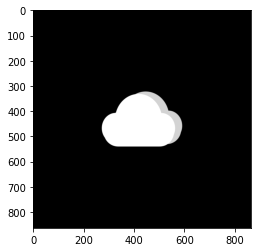
\includegraphics[width=0.5\columnwidth]{cloud-original-gs.png}}
    \caption{Cover grayscale yang digunakan untuk dilakukan steganografi}
    \label{fig:cloudbw} 
\end{figure}

Cover pada figur \ref{fig:cloudbw} akan disisipi pesan sebanyak 5000 karakter dengan jumlah bit $n = 1$. Hasil pada figure \ref{fig:result} yang didapatkan setelah melakukan steganografi secara acak dan
tidak acak.

\begin{figure}
    \centerline{
        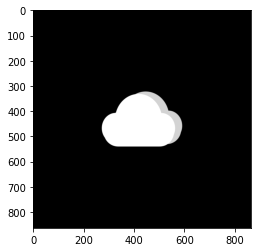
\includegraphics[width=0.4\columnwidth]{cloud-norandom-5000-gs.png}
        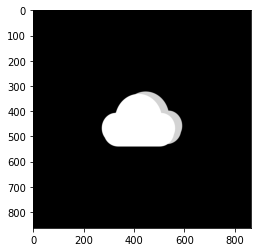
\includegraphics[width=0.4\columnwidth]{cloud-random-5000-gs.png}
    }
    \caption{Stegano-object hasil dari penyisipan data pada gambar figur \ref{fig:cloudbw}. Gambar kiri merupakan hasil dengan tanpa pengacakan dan kanan merupakan hasil dengan pengacakan}
    \label{fig:result} 
\end{figure}

Pada \emph{stego-object} tersebut tidak ditemukan perubahan yang signifikan pada cover. Akan tetapi, penempatan ini akan sangat berpengaruh pada saat melakukan steganalisis. Steganalisis dilakukan dengan
cara mengubah semua bit pada pixel menjadi bit lsb. Hal ini menimbulkan hasil pada figur \ref{fig:steganalisis5000}.

\begin{figure}
    \centerline{
        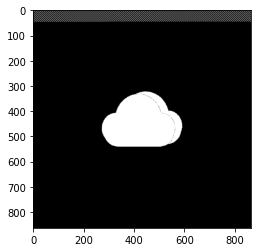
\includegraphics[width=0.4\columnwidth]{steganalisis-5000-bw.png}
        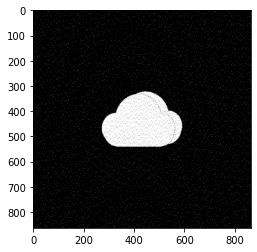
\includegraphics[width=0.4\columnwidth]{steganalisis-5000-bw-random.png}
    }
    \caption{Hasil steganalisis figur \ref{fig:result}. Gambar kiri merupakan hasil dengan tanpa pengacakan dan kanan merupakan hasil dengan pengacakan}
    \label{fig:steganalisis5000} 
\end{figure}

Bila dilihat secara lebih detail, gambar kiri menyisakan sekumpulan warna abu-abu pada awal hasil steganalisis. Akan tetapi pada gambar kanan, tidak begitu terlihat adanya perubahan pada hasil steganalisis.
Hal ini disebabkan karena pengacakan membuat data tidak berada posisi yang cukup berjauhan. Oleh karena itu, pengacakan membuat proses steganalisis lebih sulit dibandingkan dengan tanpa adanya pengacakan.

\subsection{Perbandingan Steganalisis Pada Cover Grayscale dan Berwarna}

Pada bagian ini, akan dilakukan percobaan dengan melakukan proses steganalis pada media berwarna dan media grayscale. Media berwarna yang digunakan pada proses ini adalah figur \ref{fig:cloudcol} dan cover yang digunakan
untuk media grayscale adalah figur \ref{fig:cloudbw}. Data yang akan disisipkan sebanyak 75.000 data. Pengaturan untuk konstanta $a$ diberikan nilai yang sama sebagaimana pada subbab sebelumnya.

\begin{figure}
    \centerline{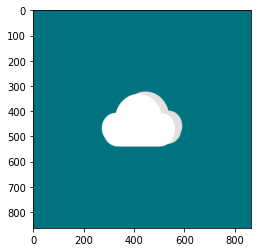
\includegraphics[width=0.5\columnwidth]{cloud-original-warna.png}}
    \caption{Cover berwarna akan digunakan dalam steganografi}
    \label{fig:cloudcol} 
\end{figure}

Hasil steganografi yang didapatkan untuk media berwarna dan grayscale ditunjukan pada figur \ref{fig:result2}.

\begin{figure}
    \centerline{
        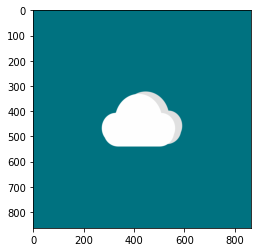
\includegraphics[width=0.5\columnwidth]{cloud-hasil-75000.png}
        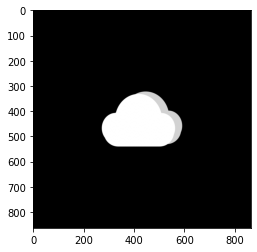
\includegraphics[width=0.5\columnwidth]{cloud-hasil-75000-s.png}
    }
    \caption{Hasil steganografi gambar pada dua buah media}
    \label{fig:result2} 
\end{figure}

Steganalisis yang dilakukan serupa degan steganalisis yang dilakukan pada subbab sebelumnya. Hasil dari steganalisis untuk gambar asli baik itu grayscale ditunjukan oleh figur \ref{fig:stegoribw} dan steganalisis untuk gambar 
berwarna asli ditunjukan oleh \ref{fig:stegoriwarna}.

\begin{figure}
    \centerline{
        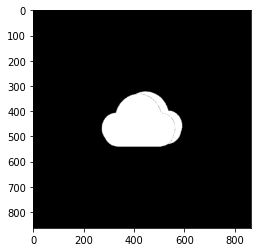
\includegraphics[width=0.5\columnwidth]{steganalisis-original-bw.png}
    }
    \caption{Hasil steganalisis gambar grayscale asli}
    \label{fig:stegoribw} 
\end{figure}

\begin{figure}
    \centerline{
        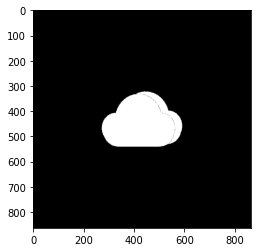
\includegraphics[width=0.3\columnwidth]{steg-warna-asli-r.png}
        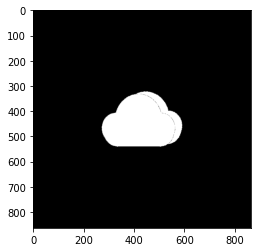
\includegraphics[width=0.3\columnwidth]{steg-warna-asli-g.png}
        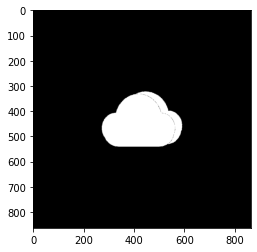
\includegraphics[width=0.3\columnwidth]{steg-warna-asli-b.png}
    }
    \caption{Hasil steganalisis gambar berwarna asli. Dimulai dari kiri hingga kanan berturut-turut menyatakan kanal R,G,dan B}
    \label{fig:stegoriwarna} 
\end{figure}

Hasil steganalisis pada \emph{stegeo-object} berwarna ditunjukan pada figur \ref{fig:result3}, sedangkan untuk media grayscale
ditunjukan pada figur \ref{fig:result4}. 

\begin{figure}
    \centerline{
        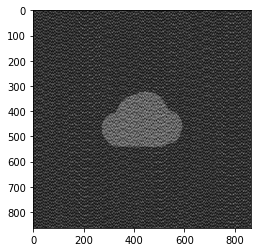
\includegraphics[width=0.5\columnwidth]{steg-75000-gs.png}
    }
    \caption{Hasil steganalisis dari \emph{stegeo-object} dengan cover grayscale}
    \label{fig:result3} 
\end{figure}

\begin{figure}
    \centerline{
        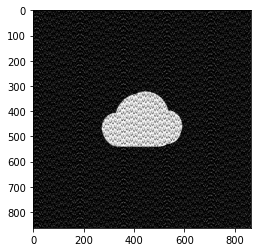
\includegraphics[width=0.3\columnwidth]{steg-75000-r.png}
        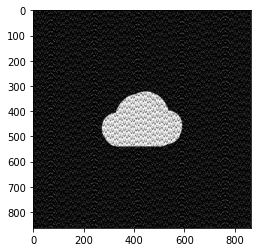
\includegraphics[width=0.3\columnwidth]{steg-75000-g.png}
        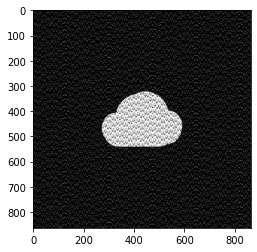
\includegraphics[width=0.3\columnwidth]{steg-75000-b.png}
    }
    \caption{Hasil steganalisis dari \emph{stegeo-object} dengan cover grayscale. Dimulai dari kiri secara berturut-turut menyatakan kanal warna R,G,dan B}
    \label{fig:result4} 
\end{figure}

Dari hasil steganalisis pada figur \ref{fig:result3} terlihat terapat banyak sekali \emph{noise} yang muncul pada hasil steganalisis visual. 
Pada hasil steganalisis pada figur \ref{fig:result4} terlihat bahwa \emph{noise} yang muncul lebih merata kepada tiap-tiap channel warna.
Hal ini menunjukan bahwa tiap data disisipkan secara menyebar pada cover berwarna untuk setiap kanal. Hal ini tentu memberikan dampak baik karena
data yang dimasukan akan lebih tersamarkan jika menganalisis menggunakan steganografi visual.

Keuntungan penggunaan kanal berwarna, cover memberikan lebih banyak ruang yang dapat disimpan pada gambar. Pada gambar dengan pixel 24-bit akan memberikan ruang 3 kali lebih
besar daripada menggunakan grayscale. Penambahan ruang juga dapat dicapai dengan menggunakan lebih dari satu bit LSB dari gambar.

\subsection{Kelebihan dan Kekurangan Sistem Steganografi Metode LSB Acak}

Sistem steganografi dengan metode LSB Acak memiliki keuntungan yaitu kemudahannya dalam implementasi. Sistem steganografi ini juga secara kasat menghasilkan \emph{stegeo-object} yang sulit untuk dibedakan dengan gambar
yang asli. Hal ini dikarenakan setiap pixel warna berubah tidak jauh dari hasil asli sehingga perubahan antara keduanya dapat tersembunyikan. Sistem ini juga dapat diintegrasikan dengan kriptografi agar menjaga data
lebih aman lagi dari sebelumnya. Pemilihan seed yang acak memiliki keuntungan yaitu menjadi kunci dari \emph{stegeo-object}.

Kekurangan dari steganografi ini adalah data yang disimpan sangat rentan terhadap perubahan kecil. Salah satu perubahan yang dapat merusak steganografi ini adalah proses kompresi gambar. Selain itu, kunci berbasis seed
sangat mudah sekali untuk dicari dengan melakukan \emph{brute-force} pada \emph{stegeo-object}. Sistem steganografi ini sangat lemah terhadap steganalisis statistik karena perubahan yang terjadi pada setiap proses akan
memberikan dampak yang besar pada hasil statistik.

\section{Kesimpulan}
Steganografi merupakan salah satu cara untuk menyembunyikan data pada sebuah cover. Steganografi memiliki banyak cara, salah satunya adalah steganografi dengan metode LSB. Metode LSB ini sangatlah sederhana dan mudah
untuk diimplementasikan pada sebuah media baik itu gambar maupun media lainnya. 

Penggunaan sistem acak dan penggunaan multi kanal dapat meningkatkan kualitas dari steganografi yang dilakukan. hal ini ditunjukan dengan hasill steganalisis visual yang menunjukan sistem acak memberikan keamanan lebih
dibandingkan tanpa pengacakan. Selain itu, penggunaan kanal secara merata dapat juga memberikan penyamaran lebih terhadap steganalisis visual sehingga lebih sulit dikenali.

\section*{Ucapan Terima Kasih}
Alhamdulillah, segala puji Allah SWT karena atas pertolongan dan rahmatnya, saya dapat menyelesaikan makalah ini. Penulis juga turut memberikan ucapan terima kasih kepada keluarga yang selalu setia untuk
memberikan motivasi dan semangat untuk dapat menyelesaikan makalah ini. Penulis juga turut mengucapkan terima kasih kepada para dosen pengampu mata kuliah Matematika Diskrit, yaitu ibu Dr. Nur Ulfa Maulidevi, S.T., M.Sc., bapak Dr. Ir.
Rinaldi Munir, M.T., dan ibu Dra. Harlili S., M.Sc. atas segala ilmunya yang telah membantu penulis dalam menyelesaikan makalah ini. Semoga dengan kebaikan yang telah diberikan, Allah akan menggantinya dengan yang lebih baik lagi.

\section*{Sumber Daya}
Segala sumber daya yang digunakan untuk membangun makalah ini dapat anda akses pada \url{https://github.com/bayusamudra5502/Matdis-Steganografi}.

\begin{thebibliography}{00}
\bibitem{b1} Munir, Rinaldi. 2019. \emph{Kriptografi Edisi Kedua}. Bandung: Penerbit Informatika 
\bibitem{b2} Munir, RInaldi. 2020. \emph{Matematika Diskrit Revisi Ketujuh}. Bandung: Penerbit Informatika
\bibitem{b3} HIdayatullah, Priyanto. 2017. \emph{Pengolahan Citra Digital Teori dan Aplikasi Nyata}. Bandung: Penerbit Informatika.
\bibitem{b4} Briant, Randal E. \& O'Hallaron, David R. 2016. \emph{Computer System A Programmer's Perspective Third Global Edition}. London: Pearson Education.
\bibitem{a1} Hull, T. E. \& Dobell, A. R. 1962. Random Number Generators. SIAM Review, 4(3), 233. Diakses pada 2021-12-04 melalui http://chagall.med.cornell.edu/BioinfoCourse/PDFs/Lecture4\\
/random\_number\_generator.pdf.
\bibitem{w1} Konsorsium World Wide Web. 2008. Web Content Accessibility Guidelines (WCAG) 2.0. Web content accessibility guidelines (WCAG) 2.0. Diakses 2021-12-04 melalui https://www.w3.org/TR/2008/REC-WCAG20-20081211/. 
\end{thebibliography}

\section*{Pernyataan}
Dengan ini saya menyatakan bahwa makalah yang saya tulis adalah tulisan saya sendiri, bukan sanduran, ataupun terjemahan dari makalah orang lain, dan bukan plagiasi.


\vspace{20px}
\hspace*{\fill} Cimahi, 14 Desember 2021

\vspace{30px}
\hspace*{\fill} Bayu Samudra - 13520128

\end{document}
